\section{}
% Air at 900 kPa and 400 K enters a converging nozzle with a negligible velocity. 
% The throat area of the nozzle is 10 cm2
% . Approximating the flow as isentropic, 
% calculate and plot the exit pressure, the exit velocity, and the mass flow rate 
% versus the back pressure 𝑃𝑏 for 0.9 ≥ 𝑃𝑏 ≥ 0.1 MPa. (Note: Use MATLAB to 
% plot the results)

\textit{Air at $900 kPa$ and $400 K$ enters a converging nozzle with a negligible velocity. The throat area of the nozzle is $10 cm^2$. Approximating the flow as isentropic, calculate and plot the exit pressure, the exit velocity, and the mass flow rate versus the back pressure $P_b$ for $0.9 \geq P_b \geq 0.1 MPa$. (Note: Use MATLAB to plot the results)}

\textbf{Solution}

Assume
\begin{itemize}
    \item The flow is steady, adiabatic, and one dimensional
    \item Isentropic flow
    \item Air is an ideal gas 
\end{itemize}
First find the critical pressure,
\begin{align*}
    P^\star &= P \left( \frac{2}{k+1} \right)^{\frac{k}{k-1}} \\
    &= 900 \left( \frac{2}{1.4+1} \right)^{\frac{1.4}{0.4}} \\
    &= 900 \times 0.5283 \\
    &= 475.4536 \text{ kPa}
\end{align*}
Recall that exit pressure, $P_e$ is described as 
\begin{align*}
    P_e &= \begin{cases}
        P_b, & P_b \geq P^\star \\
        P^\star, & P_b < P^\star
    \end{cases}
\end{align*}
so, 
\begin{empheq}[box=\fbox]{align*}
    P_e &= \begin{cases}
        P_b, & P_b \geq 475.4536 \\
        475.4536, & P_b < 475.4536
    \end{cases}
\end{empheq}
Assuming air is ideal,
\begin{gather*}
    c_p T_0 = c_p T + \frac{V^2}{2} \\
    \implies V = \sqrt{2c_p(T_0 - T)}
\end{gather*}
Let is consider the case where $P_b < P^\star$. Then, $P_e = 475.4536$ kPa. Solving for $T_e$,
\begin{align*}
    T_e &= T_0 \left( \frac{P_e}{P_0} \right)^{\frac{k-1}{k}} \\
    &= 400 \left( \frac{475.4536}{900} \right)^{\frac{0.4}{1.4}} \\
    &= 333.33 \text{ K}
\end{align*}
Then,
\begin{align*}
    V &= \sqrt{2 \cdot 1.005 \cdot 10^3 \cdot (400 - 333.33)} \\
    &= 366.069 \text{ m/s}
\end{align*}
For the case where $P_b \geq P^\star$, $P_e = P_b$. Then,
\begin{align*}
    T_e &= T_0 \left( \frac{P_e}{P_0} \right)^{\frac{k-1}{k}} \\
    &= 400 \left( \frac{P_b}{900} \right)^{\frac{0.4}{1.4}} \\
    &= 57.278 P_b^{0.286}
\end{align*}
Then,
\begin{align*}
    V &= \sqrt{2 \cdot 1.005 \cdot 10^3 \cdot (400 - 57.278 P_b^{0.286})} \\
    &= 44.83 \sqrt{400 - 57.278 P_b^{0.286}}
\end{align*}
So,
\begin{empheq}[box=\fbox]{align*}
    V &= \begin{cases}
        366.069, & P_b < 475.4536 \text{ kPa} \\
        44.83 \sqrt{400 - 57.278 P_b^{0.286}}, & P_b \geq 475.4536 \text{ kPa}
    \end{cases}
\end{empheq}
The mass flow rate is given by 
\begin{align*}
    \dot{m} &= \rho_e A V 
\end{align*}
By ideal gas law,
\begin{align*}
    \rho_e &= \frac{P_e}{RT_e} \\
    &= \frac{P_e}{0.287 \cdot T_e}
\end{align*}
Then for $P_b < 475.4536$ kPa,
\begin{align*}
    \rho_e &= \frac{475.4536}{0.287 \cdot 333.33} \\
    &= 4.9699479573 \text{ kg/m}^3
\end{align*}
and for $P_b \geq 475.4536$ kPa,
\begin{align*}
    \rho_e &= \frac{P_b}{0.287 \cdot 57.278 P_b^{0.286}} \\
    &= \frac{1}{0.287 \cdot 57.278 P_b^{0.286 - 1}} \\
    &= \frac{1}{16.439 P_b^{-0.7143}}
\end{align*}
Then,
\begin{empheq}[box=\fbox]{align*}
    \dot{m} &= \begin{cases}
        4.9699479573 \cdot 10 \times 10^{-4} \cdot 366.069, & P_b < 475.4536 \text{ kPa} \\
        \frac{1}{16.439 P_b^{-0.7143}} \cdot 10 \times 10^{-4} \cdot 44.83 \sqrt{400 - 57.278 P_b^{0.286}}, & P_b \geq 475.4536 \text{ kPa}
    \end{cases}
\end{empheq}
This gets way too complicated, so I'll just make a table using Excel.
\begin{table}[H]
    \centering
    \begin{tabular}{ccccccc}
        \toprule
        $P_b$ & $P_e$ & $T_e$ & $V_e$ & $\rho_e$ & $\dot{m}$ \\
        (kPa) & (kPa) & (K) & (m/s) & (kg/m$^3$) & (kg/s) \\
        \midrule
        100 & 100 & 475.4536 & 366.069 & 4.9699 & 1.8193 \\
        200 & 200 & 475.4536 & 366.069 & 4.9699 & 1.8193 \\
        300 & 300 & 475.4536 & 366.069 & 4.9699 & 1.8193 \\
        400 & 400 & 475.4536 & 366.069 & 4.9699 & 1.8193 \\
        500 & 500 & 333.3333 & 366.0601 & 4.9699 & 1.8193 \\
        600 & 600 & 356.2445 & 296.5611 & 5.8684 & 1.7403 \\
        700 & 700 & 372.2853 & 236.0225 & 6.5515 & 1.5463 \\
        800 & 800 & 386.7631 & 163.1142 & 7.2071 & 1.1756 \\
        900 & 900 & 400 & 0 & 7.8397 & 0 \\
        \bottomrule
    \end{tabular}
\end{table}
Plotting the results with Matplotlib \cite{matplotlib}, Figures \ref{fig:P_e_vs_P_b}, \ref{fig:V_e_vs_P_b}, and \ref{fig:m_vs_P_b} are obtained.
\begin{figure}[H]
    \centering
    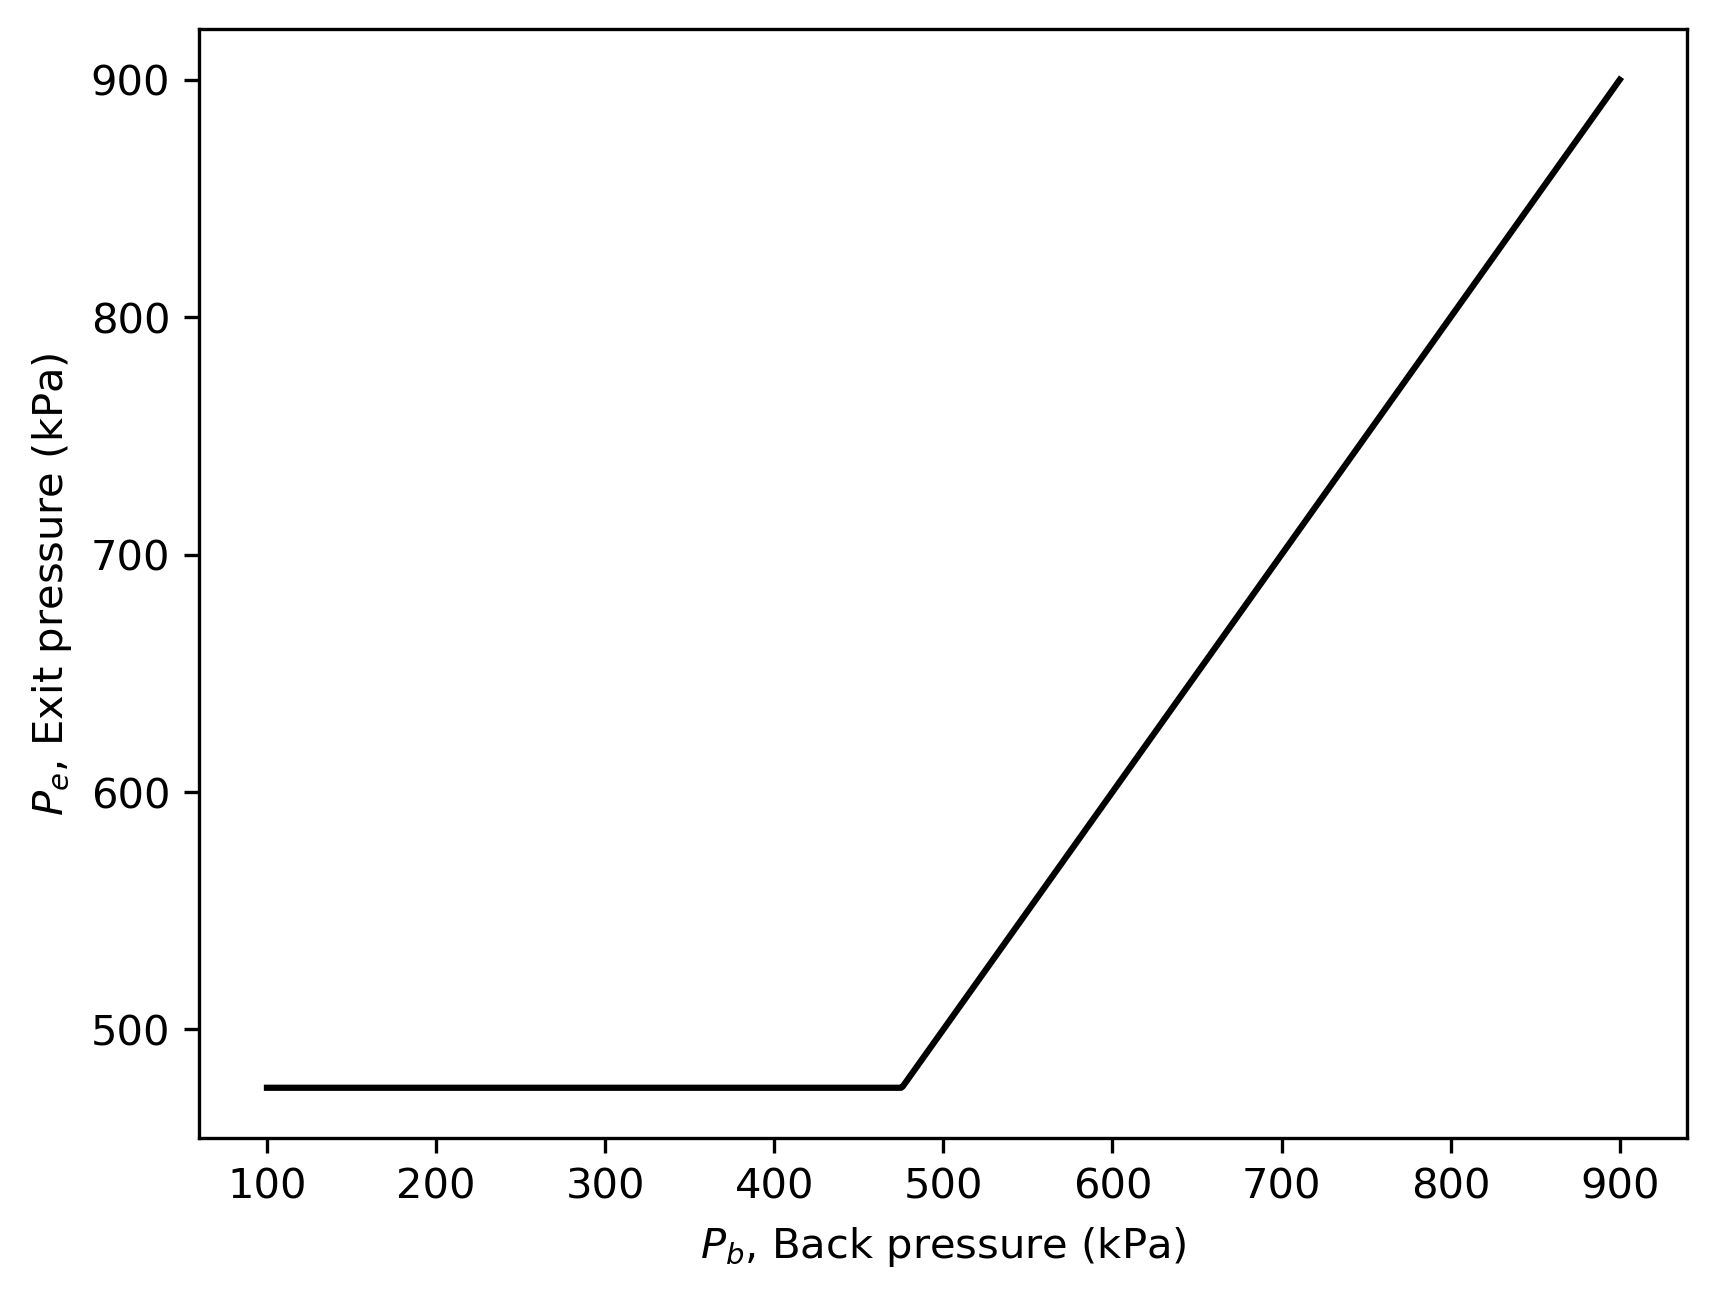
\includegraphics[width=0.7\textwidth]{Questions/Figures/P_e_vs_P_b.png}
    \caption{Exit Pressure vs. Back Pressure}
    \label{fig:P_e_vs_P_b}
\end{figure}
\begin{figure}[H]
    \centering
    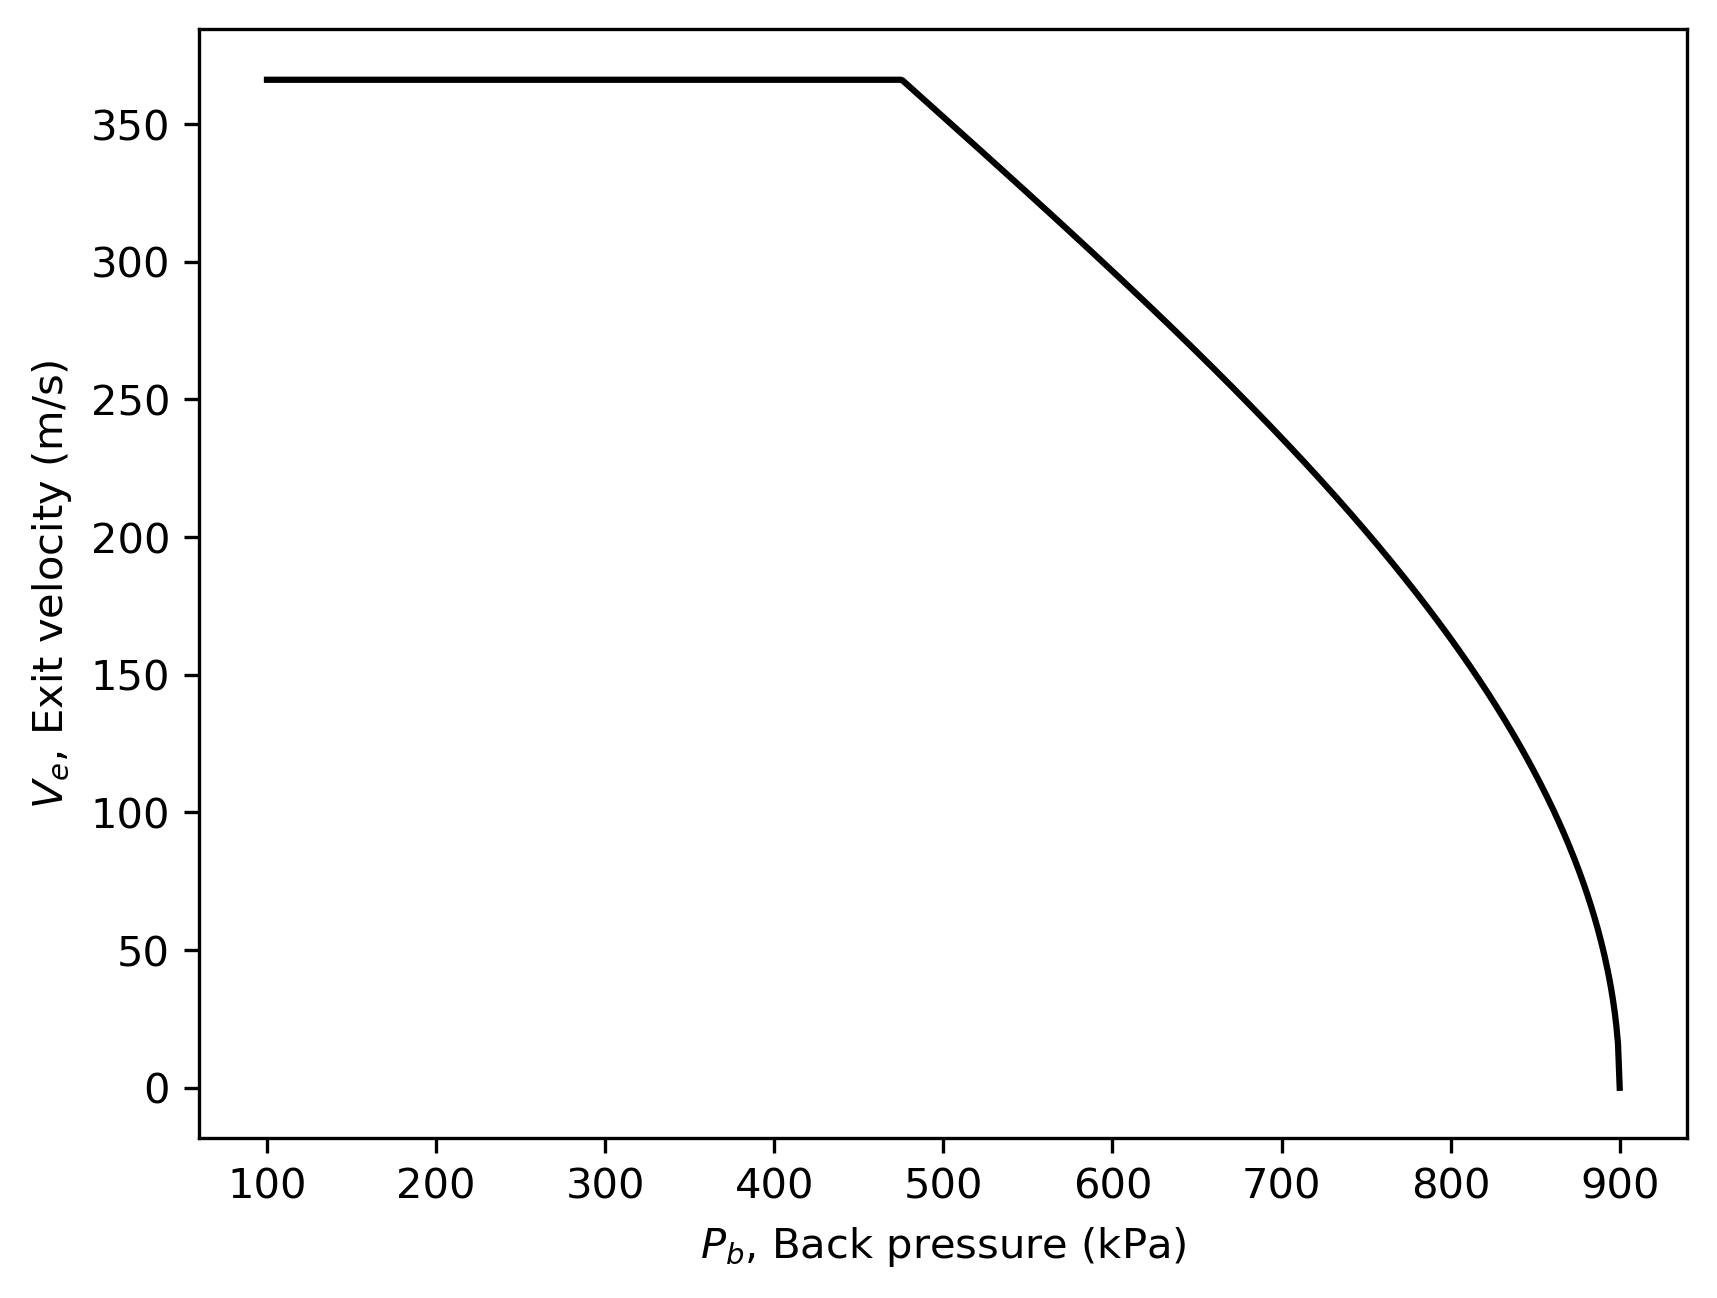
\includegraphics[width=0.7\textwidth]{Questions/Figures/V_e_vs_P_b.png}
    \caption{Exit Velocity vs. Back Pressure}
    \label{fig:V_e_vs_P_b}
\end{figure}
\begin{figure}[H]
    \centering
    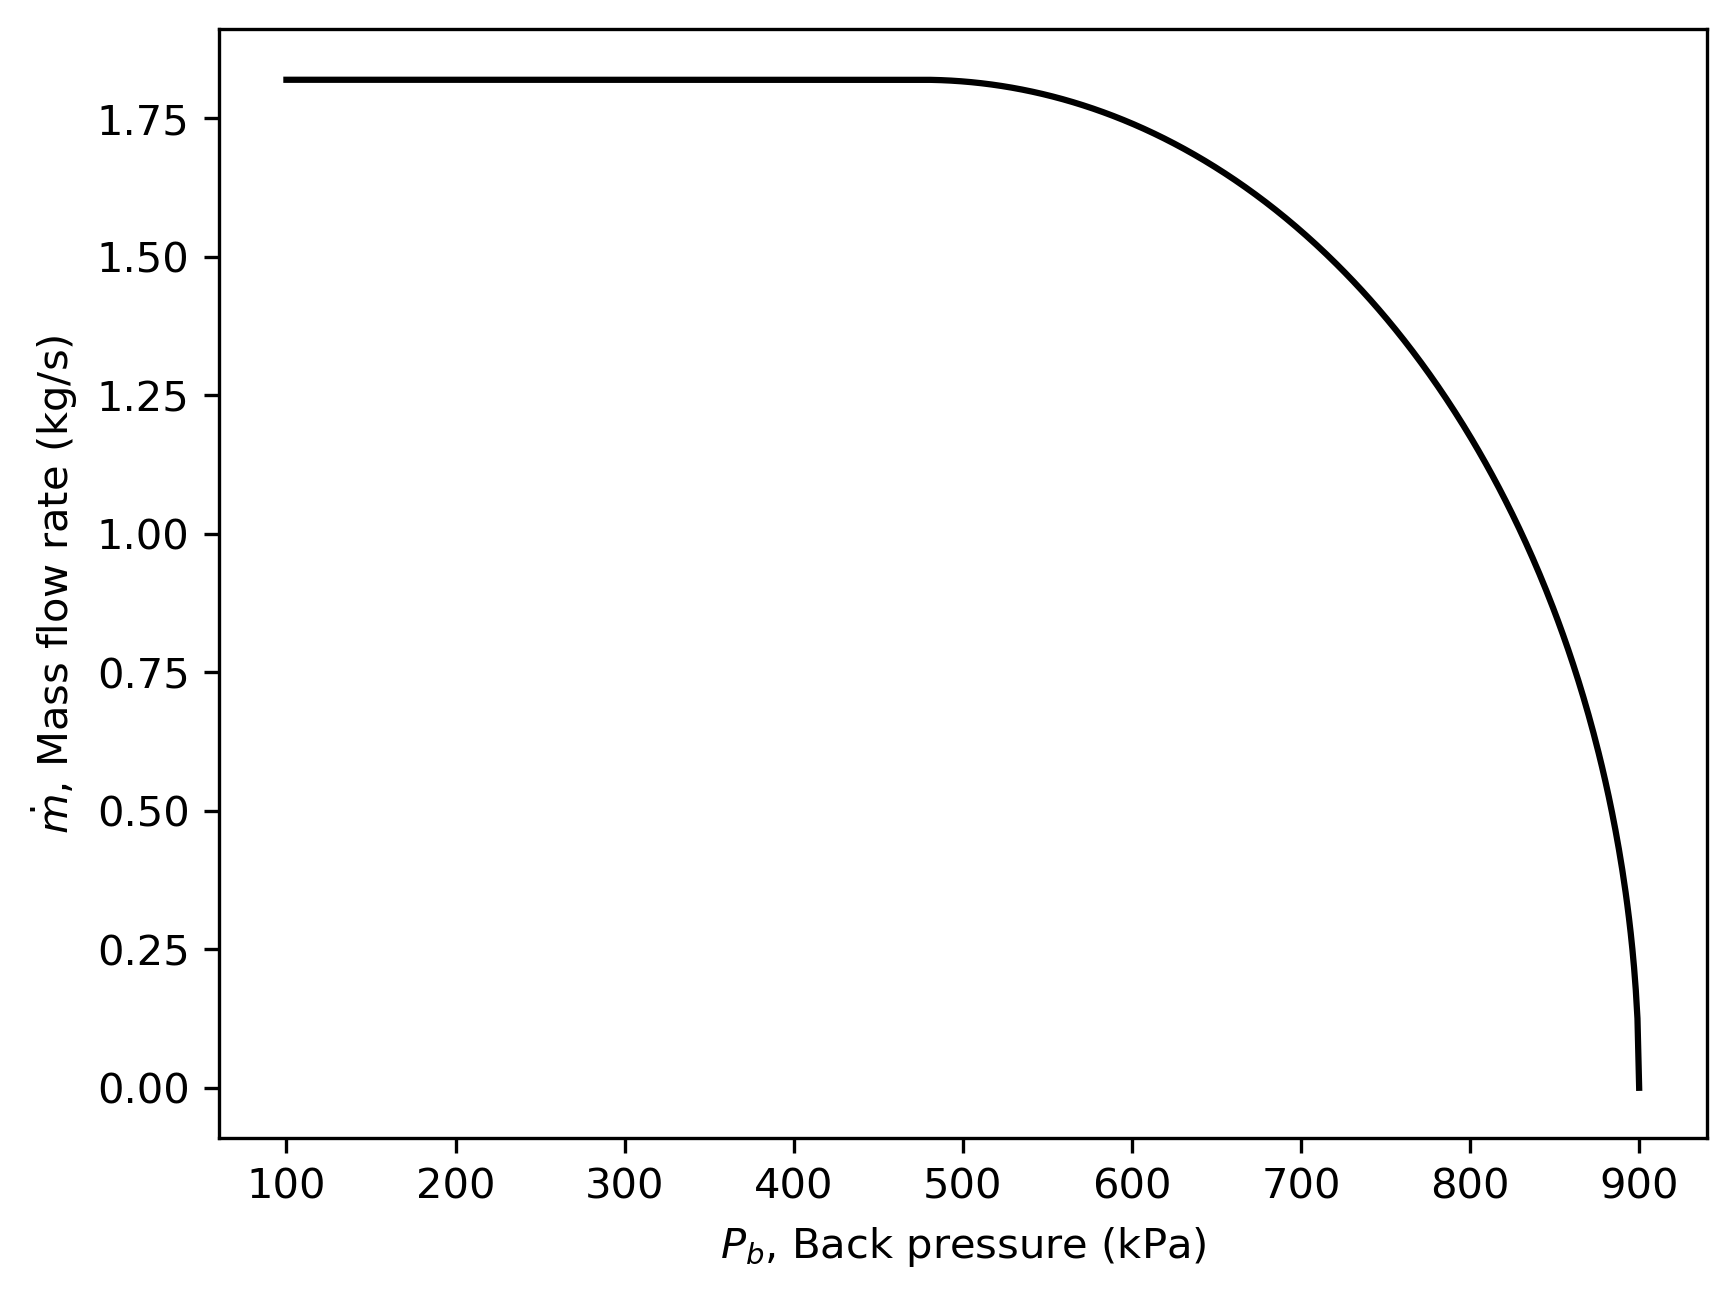
\includegraphics[width=0.7\textwidth]{Questions/Figures/m_vs_P_b.png}
    \caption{Mass Flow Rate vs. Back Pressure}
    \label{fig:m_vs_P_b}
\end{figure}
